\begin{minipage}{0.5\linewidth}
\subsection{UMTS Ziele}
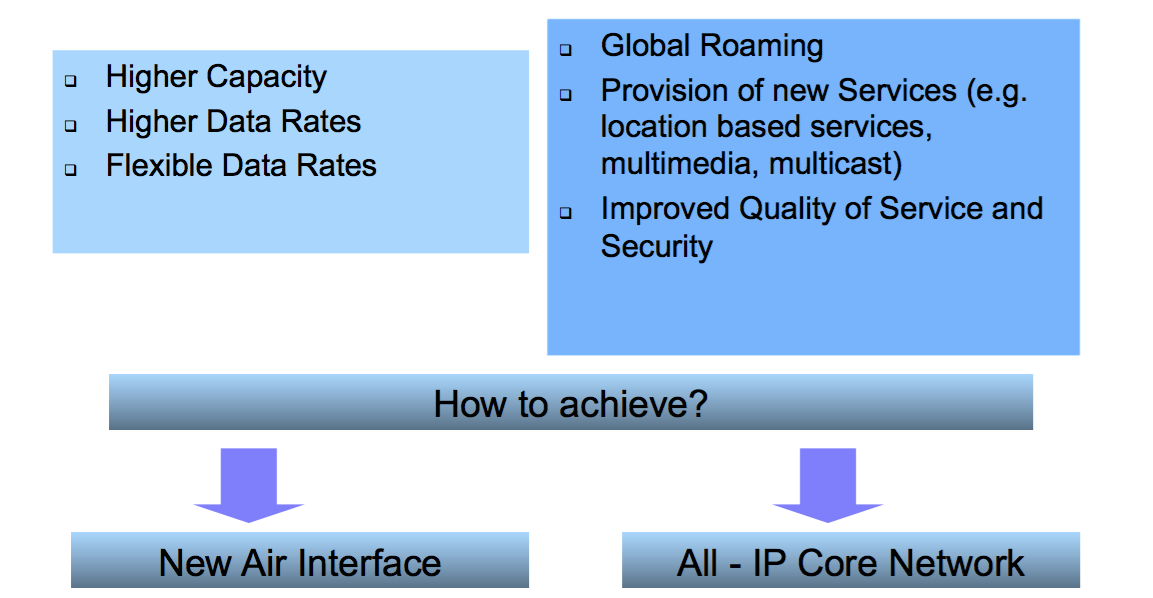
\includegraphics[width = \linewidth]{./Pics/UMTS}
\end{minipage}
\begin{minipage}{0.5\linewidth}
\subsection{UMTS Entscheidungfaktoren}
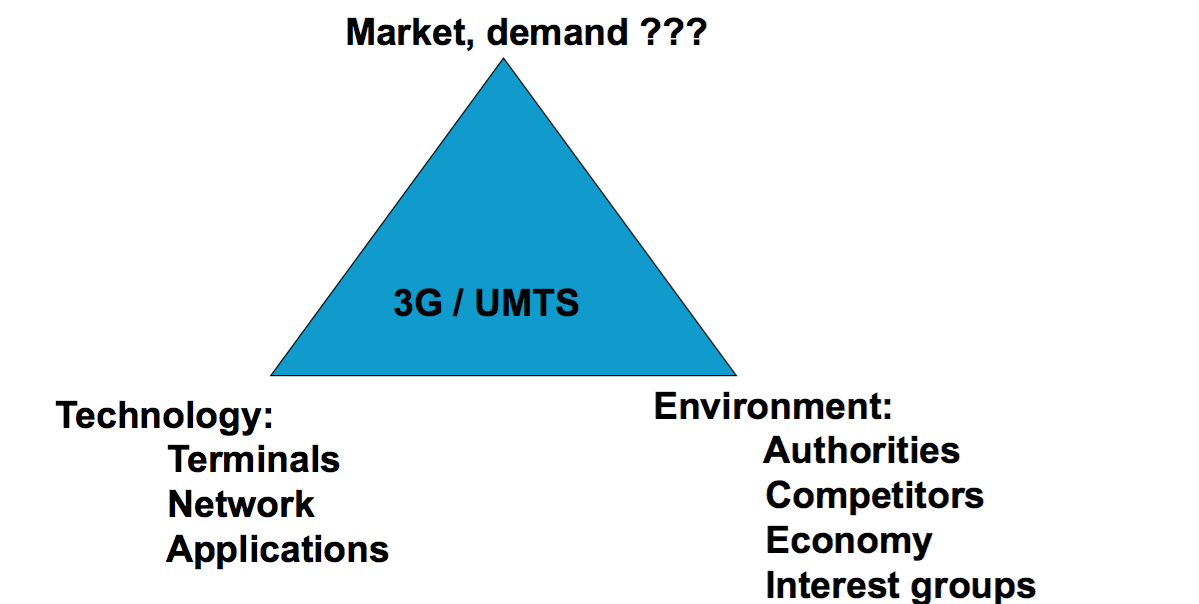
\includegraphics[width = \linewidth]{./Pics/UMTS3}
\end{minipage}

\begin{minipage}{0.5\linewidth}
\subsection{UMTS Verspricht}
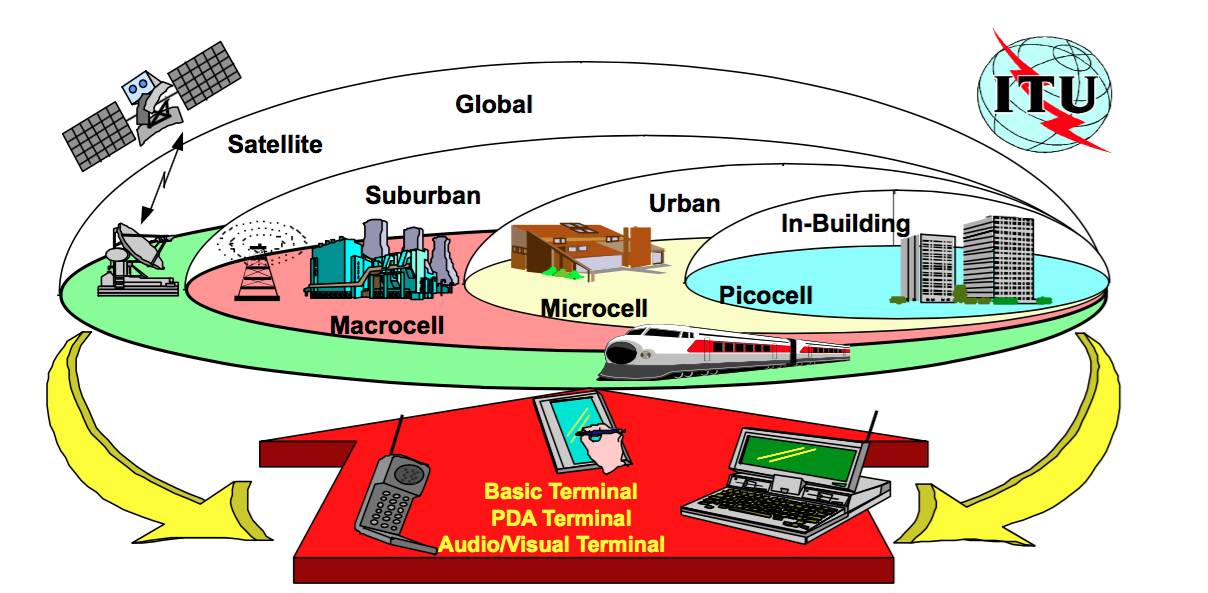
\includegraphics[width = \linewidth]{./Pics/UMTS2}
\end{minipage}
\begin{minipage}{0.5\linewidth}
\subsection{UMTS Klärende Fragen}
\begin{itemize}
\item Welche Netzelemente sind erforderlich ? 
\begin{itemize}
\item System Architecture
\item System Components and Identifiers
\end{itemize}
\item Wie Kommunizieren die Netzelemente ?
\begin{itemize}
\item Protocols and Logical Channels
\end{itemize}
\item Was sind die erforderlichen Netzprozeduren ? 
\begin{itemize}
\item Establish, Maintain and Release Communication Links
\item Provide sufficient Quality of Service
\end{itemize}
\item Wie wird der erforderliche QoS sichergestellt?
\begin{itemize}
\item Radio Access Network Design (im speziellen PHY)
\end{itemize}
\end{itemize}
\end{minipage}

\subsection{Evolution von GPRS zu UMTS}
\begin{minipage}{0.45\linewidth}
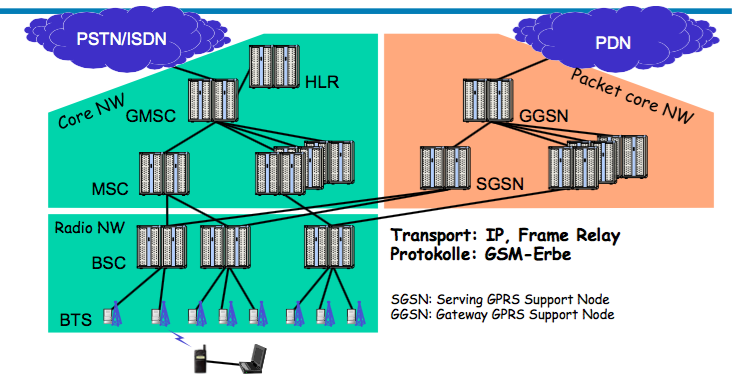
\includegraphics[width = \linewidth]{./Pics/UMTS4}
\end{minipage}
\begin{minipage}{0.1\linewidth}
$\Rightarrow$
\end{minipage}
\begin{minipage}{0.45\linewidth}
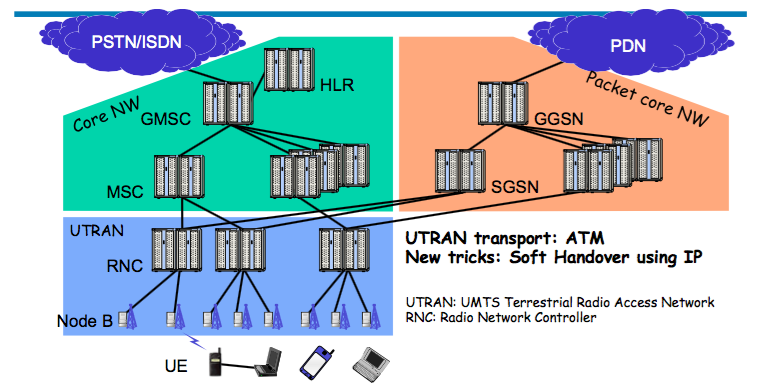
\includegraphics[width = \linewidth]{./Pics/UMTS5}
\end{minipage}

\subsection{UMTS Architektur}
\begin{minipage}{0.5\linewidth}
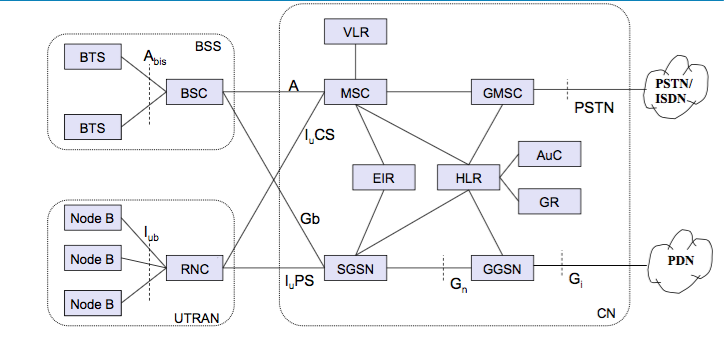
\includegraphics[width = \linewidth]{./Pics/UMTSArch} \\
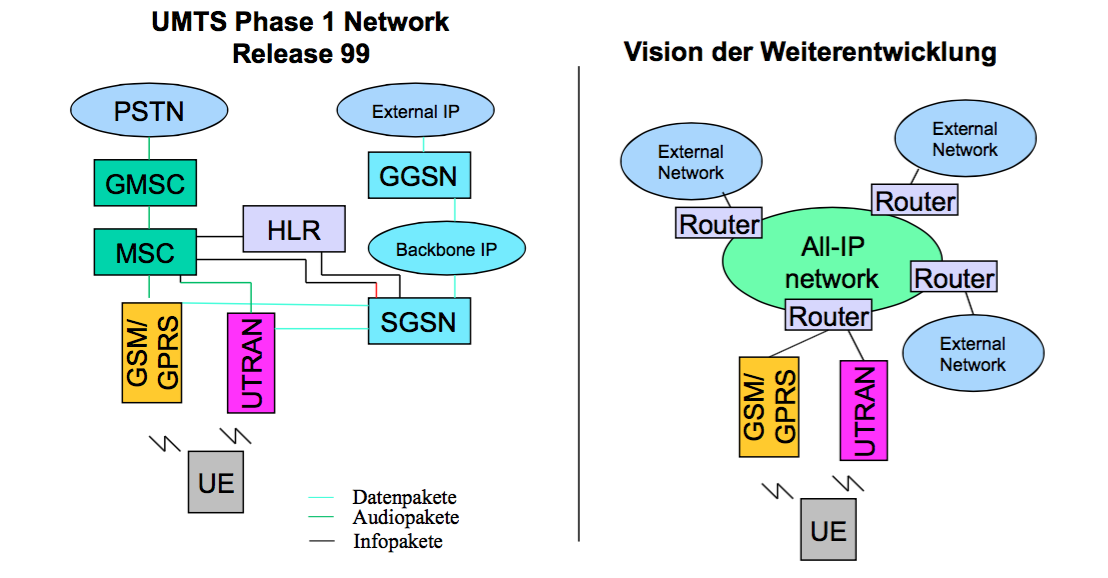
\includegraphics[width = \linewidth]{./Pics/UMTSArch3}
\end{minipage}
\begin{minipage}{0.5\linewidth}
\begin{itemize}
\item Das Core Network (CN) und auch das Interface $I_u$ sind aufgeteilt in zwei logische Domänen:
\item Circuit Switched Domain (CSD)
\begin{itemize}
\item Circuit Switched Dienst inkl. Signalisation
\item Ressourcen -Reservation beim Verbindungsaufbau
\item GSM Komponenten (MSC, GMSC, VLR)
\item $I_uCS$
\end{itemize}
\item Packet Swiched Domain (PSD)
\begin{itemize}
\item GPRS Komponenten (SGSN, GGSN)
\item $I_uPS$
\end{itemize}
\item Release 99 benutzt das GSM/GPRS Netzwerk und ergänzt das Netzwerk um ein neues Radio Access Network dem UTRAN
\begin{itemize}
\item Spart Geld...
\item Schnellere Entwicklung
\item Nicht so flexibel 
\end{itemize}
UE (User Equipment)
\begin{itemize}
\item Mobile Equipment: Mobiles Endgerät, das via Uu mit dem Netz kommuniziert
\item UMTS SIM: Smartcard, die die subscriber identity enthält, die Authentifikation durchführt und die Authentifikations- und Encryption-Schlüssel speichert.
\end{itemize}
\item UTRAN (UMTS Terrestrial Radio Access Network)
\begin{itemize}
\item Node B (Basestation = Antenne): Konvertiert den Datenfluss zwischen Iub und Uu interface (vergleichbar zur BTS im GSM Netzwerk)
\item Radio Network Controll (RNC): besitzt und kontrolliert die Radioressourcen von allen Node-Bs in seiner Domäne (vergleichbar zur BSC in GSM). Verwaltet die Codes
\end{itemize}
\end{itemize}
\end{minipage}

\begin{minipage}{0.5\linewidth}
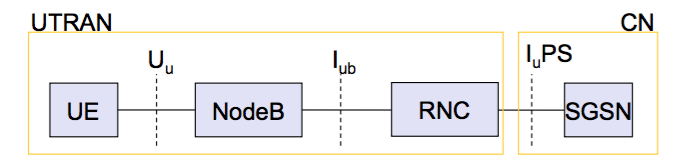
\includegraphics[width = \linewidth]{./Pics/UMTSArch2}
\end{minipage}
\begin{minipage}{0.5\linewidth}
\begin{itemize}
\item CN (Core Network)
\begin{itemize}
\item HLR, MSC, VLR, GMSC, SGSN, GGSN (vergleichbar zum GPRS)
\item Neue Schnittstellen (interfaces, auch Reference Points) sind standardisiert worden (IuPS, IuCS)
\end{itemize}
\end{itemize}
\end{minipage}

\begin{minipage}{0.5\linewidth}
\subsubsection{Release 4}
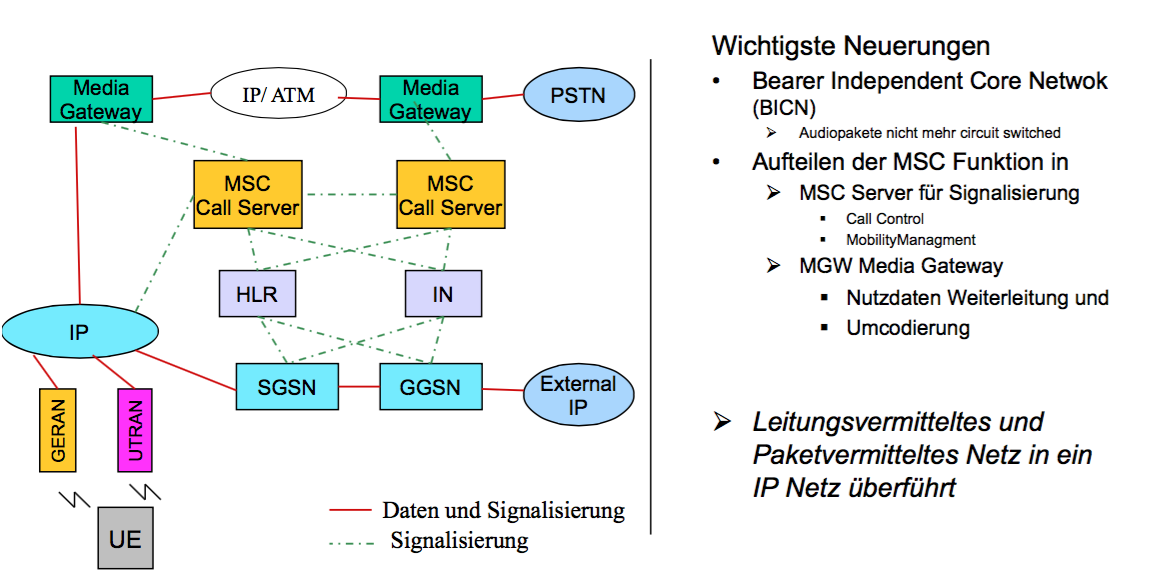
\includegraphics[width = \linewidth]{./Pics/UMTSArch4}
\end{minipage}
\begin{minipage}{0.5\linewidth}
\subsubsection{Release 5}
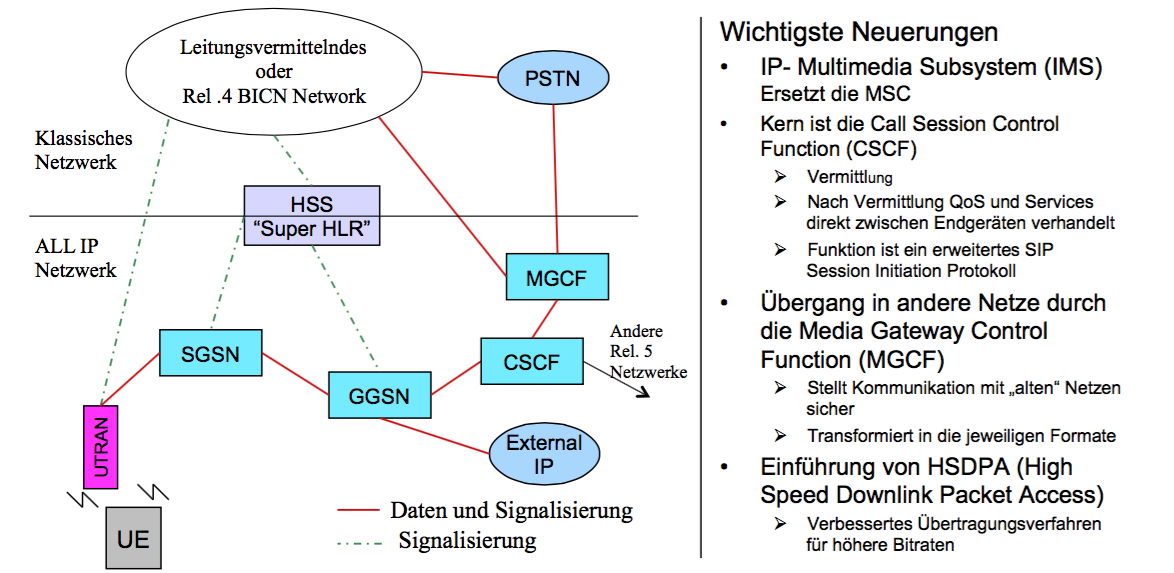
\includegraphics[width = \linewidth]{./Pics/UMTSArch5}
\end{minipage}

\begin{minipage}{0.5\linewidth}
\subsubsection{Release 6}
\begin{itemize}
\item Mit der Ergänzung des HSUPA zum bereits existierenden HSDPA sind jetzt Übertragungsraten im Mbit/s Bereich in beide Richtungen möglich. Zusammengefasst wird das ganze auch als HSPA bezeichnet

\subsubsection{Release 8}
\begin{itemize}
\item LTE $\rightarrow$ eigenes Kapitel
\item HSPA+ $\rightarrow$ höhere Übertragungsraten durch Bündelung zweier Kanäle bis 42Mbit/s
\item Verbesserung der Performance-Regelung
\item Einführung von Femto-Zellen zum Einsatz im privaten Bereich mit minimaler Reichweite
\end{itemize}
\end{itemize}

\subsubsection{Release 10}
\begin{itemize}
\item LTE Adcanced
\end{itemize}
\end{minipage}
\begin{minipage}{0.5\linewidth}
\subsubsection{Release 7}
\begin{itemize}
\item HSPA+
\begin{itemize}
\item Erhöhung der Datenrate durch die Verwendung mehrerer Antennen: Multiple Input Multiple Output (MIMO) Übertragung
\item Einführung einer 64 Quadrature Amplituden Modulation im Downlink
\item Übertragungsraten: DL 28 Mbit/s, UL bis 11.5 Mbit/s
\end{itemize}
\item CPC Continous Packet Connectivity
\begin{itemize}
\item Minimiert die Stromaufnahme durch intelligentere Protokolle der Verbindungsregelung
\end{itemize}
\end{itemize}
\subsubsection{Release 9}
\begin{itemize}
\item nur kleine Korrekturen zu Release 8
\end{itemize}
\end{minipage}

\subsection{UMTS Protocol Stack}
\begin{minipage}{0.5\linewidth}
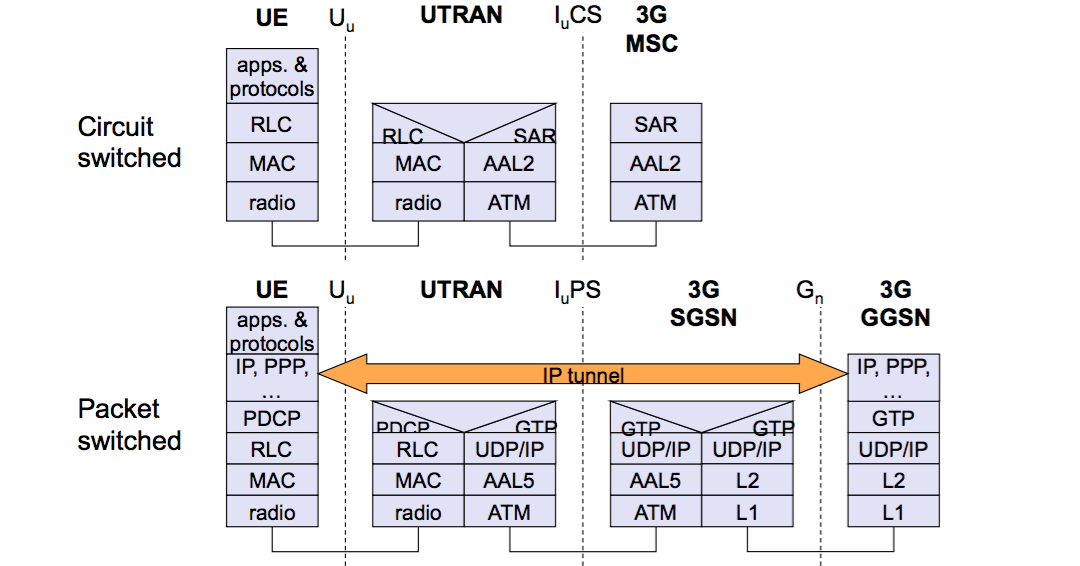
\includegraphics[width = \linewidth]{./Pics/UMTSArch6}
\end{minipage}
\begin{minipage}{0.5\linewidth}
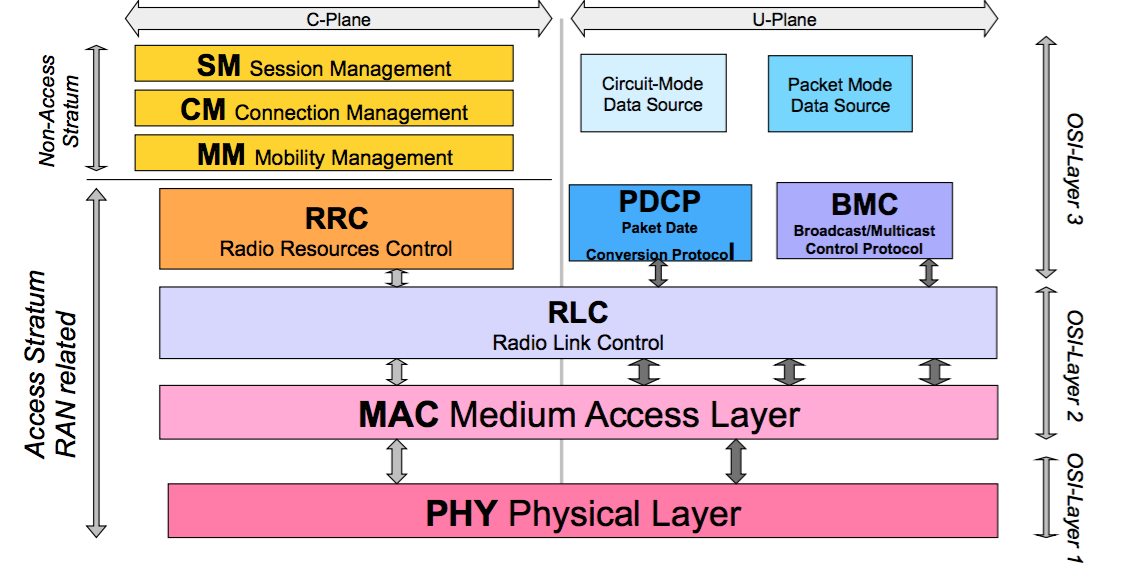
\includegraphics[width = \linewidth]{./Pics/UMTSStack}
\end{minipage}

\begin{minipage}{0.4\linewidth}
\subsubsection{RRC (Radio Resource Control)}
\begin{itemize}
\item Initial Cell Selection
\item Admission Control
\item Congestion Control
\item System Information Broadcasting
\item Paging
\item Control of Security Functions
\item Handover (Intra RNC)
\item URTAN Registration Area Update
\item Establish, Control and Release of RRC connection
\item Establish, Control and Release of Transport and Physical Channels
\item Control UE measurement reports
\end{itemize}
\end{minipage}
\begin{minipage}{0.25\linewidth}
\subsubsection{RLC (Radio Link Control)}
\begin{itemize}
\item Segmentation and Reassembly 
\item Concatenation
\item Padding
\item Duplicate Detection
\item In-Sequence delivery
\item Error Correction
\item Flow Control
\end{itemize}
\end{minipage}
\begin{minipage}{0.35\linewidth}
\subsubsection{MAC (Medium Access Control)}
\begin{itemize}
\item Mapping between logical and transport Channels
\item Dynamic Transport Format Selection
\item Dynamic Transport Type Switching
\item Priority Handling between Data Flows
\item Identification of UEs on common transport channels
\item Multiplexing/Demultiplexing Scheduling
\item Radio Channel Encryption
\end{itemize}
\end{minipage}

\subsection{UMTS Channels}
\begin{minipage}{0.5\linewidth}
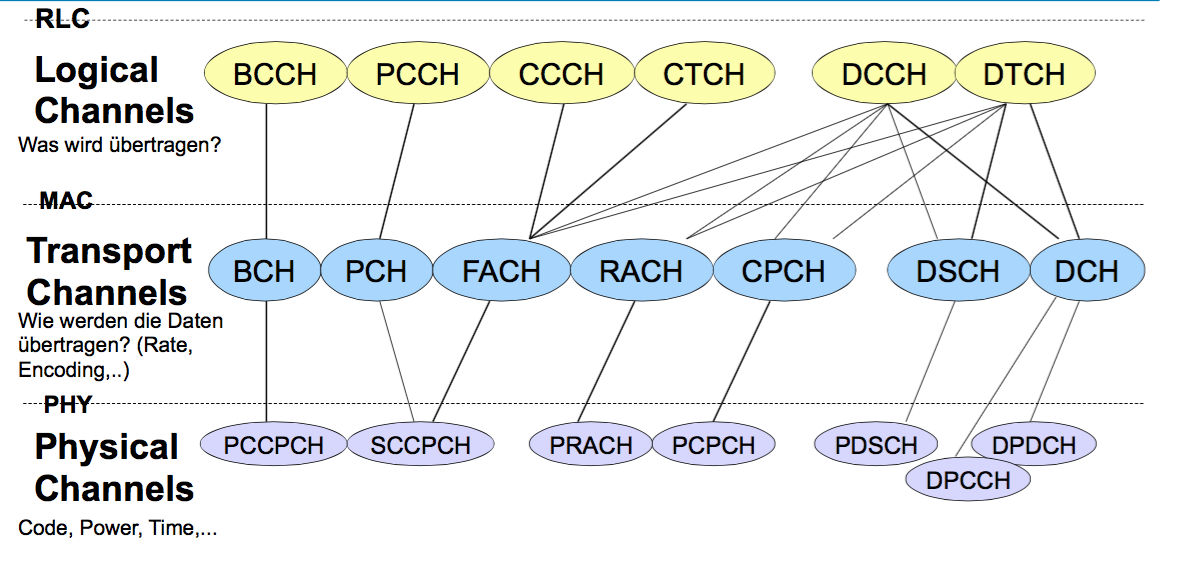
\includegraphics[width = \linewidth]{./Pics/UMTSCH}
\end{minipage}
\begin{minipage}{0.5\linewidth}
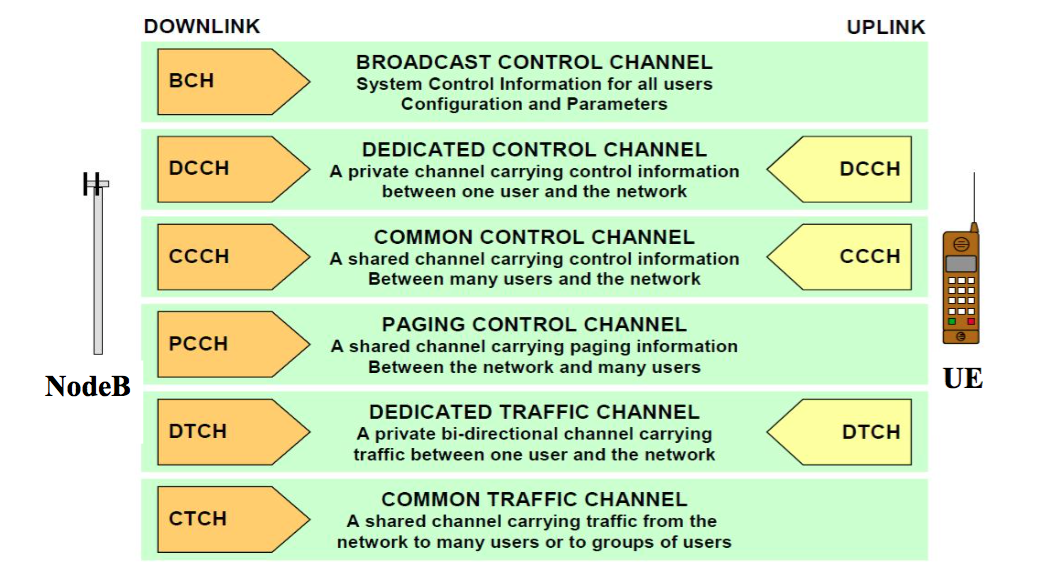
\includegraphics[width = \linewidth]{./Pics/UMTSCH2}
\end{minipage}

\subsubsection{WCDMA Wide Code Division MultipleAccess}
\begin{minipage}{0.5\linewidth}
\begin{itemize}
\item Traditionelle Funkkommunikation fokusiert auf Schmalbandsignalen (z.B. FM Radio)
\item Spreizband nimmt ein Schmalbandiges Signal und verteilt die Signalpower auf ein grösseres Band
\item Wenn Sender und Empfänger mit der gleichen Technologie ausgestattet sind, kann das Signal beim Empfänger wieder in ein Schmalbandsignal umgewandelt werden
\item Für Schmalband-Empfänger sieht es wie Rauschen aus 
\end{itemize}
\end{minipage}
\begin{minipage}{0.5\linewidth}
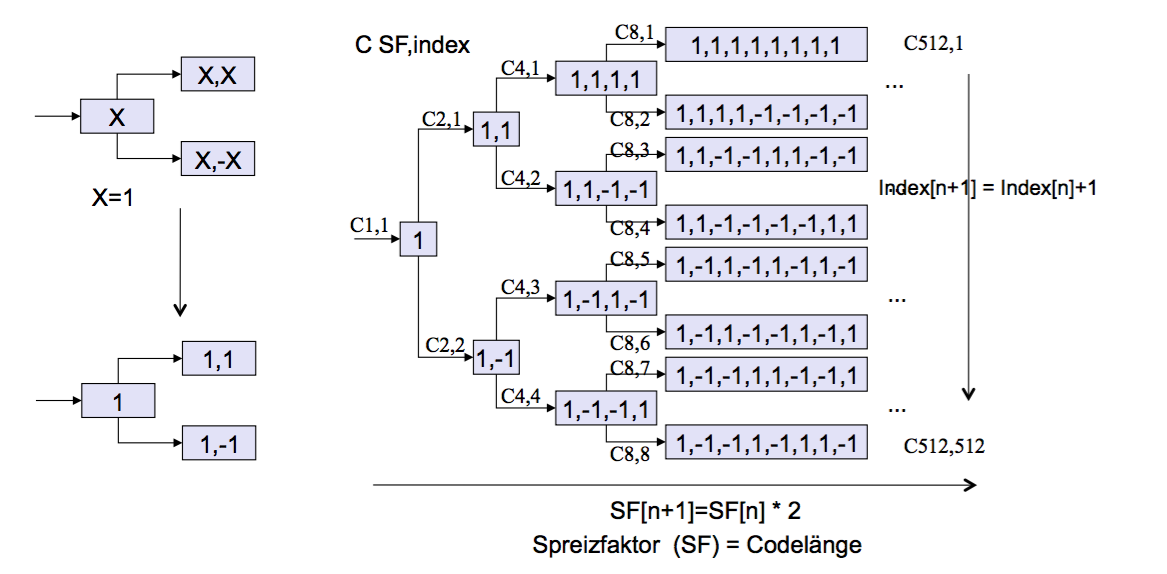
\includegraphics[width = \linewidth]{./Pics/UMTSCH3}
\end{minipage}

\subsection{Zellplanung}
\begin{minipage}{0.3\linewidth}
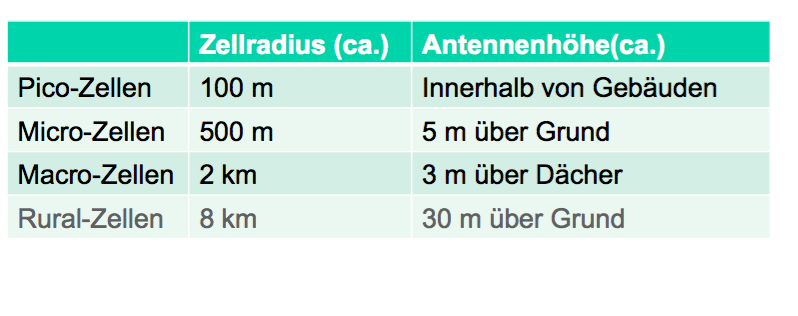
\includegraphics[width = \linewidth]{./Pics/UMTSZell}
\end{minipage}
\begin{minipage}{0.7\linewidth}
\begin{itemize}
\item Alle Zellen arbeiten auf der gleichen Frequenz durch WCDMA
\item Daher vereinfachte Zellplanung
\item Aber Interferenzplanung:
\begin{itemize}
\item Sendeleistung der Nachbarstationen
\item Komplex Regelung der Sende-Leistung der MS (1500 pro S pro MS)
\item Hauptaufgabe Interferenzeplanung
\end{itemize}
\item Kein Timing Advance durch individuelle Scrampling Codes der Teilnehmer
\item Zellgrösse $\rightarrow$ Zellatmung
\begin{itemize}
\item durch das Interferenzniveau kann die Zelle kleiner werden
\end{itemize}
\end{itemize}
\end{minipage}